\section{Auswertung}
\label{sec:Auswertung}
\subsection{Überprüfung der Braggbedingung}
Zur Überprüfung der Braggbedingung wurde der Kristallwinkel auf $\SI{14}{\degree}$ eingestellt.
Die Messdaten befinden sich in Tabelle \ref{tab:bragg}.

\begin{table}
  \centering
  \caption{Messwerte zur Überprüfung der Braggbedingung.}
  \label{tab:bragg}
  \begin{tabular}[t]{c@{} S[table-format=2.1] S[table-format=3.0] | }
   \toprule
     {$2\cdot \theta \, / \, \si{\degree}\:\:$} & {$\text{Counts} \, /  \, \si{\per\second}$} \\\midrule
     \csvreader[no head,
     late after line=\\,
     late after last line=\\\bottomrule,
     filter test={\ifnumless{\thecsvinputline}{22}}]%
     {data/braggbedingung.csv}{}%
     {$\SI{\csvcoli}{}$ & $\SI{\csvcolii}{}$}%
   \end{tabular}
   \begin{tabular}[t]{ | c@{} S[table-format=2.1] S[table-format=3.0]}
    \toprule
      {$2\cdot \theta \, / \, \si{\degree}\:\:$} & {$\text{Counts} \, /  \, \si{\per\second}$} \\\midrule
     \csvreader[filter test={\ifnumgreater{\thecsvinputline}{21}},
     late after line=\\,
     late after last line=\\\bottomrule]%
     {data/braggbedingung.csv}{}%
    {$\SI{\csvcoli}{}$ & $\SI{\csvcolii}{}$}%
  \end{tabular}
\end{table}
\begin{figure}
  \centering
  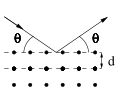
\includegraphics{bragg.pdf}
  \caption{Plot zur Überprüfung der Bragg-Bedingung.}
  \label{fig:bragg}
\end{figure}

Das Maximum der Intensität lässt sich aus dem Plot zu $\SI{13.9}{\degree}$ bestimmen und weicht um $\SI{0.7}{\percent}$ vom eingestellten Winkel ab.

\FloatBarrier
\subsection{Das Emissionsspektrum einer Cu-Röntgenröhre}

Die gemessenen Winkel und die entsprechenden Counts pro Sekunde sind in der Tabelle \ref{tab:Emissionsspektrum} zusammengefasst.
Diese wurden graphisch in Abbildung \ref{fig:Emissionsspektrum} dargestellt.
Dort können die K$_\alpha$ und K$_\beta$ abgelesen werden.

\begin{figure}
  \centering
  \includegraphics{build/emission.pdf}
  \caption{Graphische Darstellung der Messergebnisse und kenntlich machen der K$_\alpha$- und K$_\beta$-Linien und des Bremsberges.}
  \label{fig:Emissionsspektrum}
\end{figure}

\begin{table}
  \centering
  \caption{Die zu den entsprechenden Winkeln gemessenen Counts.}
  \label{tab:Emissionsspektrum}
  \begin{tabular}[t]{c@{} S [table-format=2.1] S [table-format=4.0] |}
    \toprule
      {$2 \cdot \theta \, / \, \si{\degree}\:\:$} & {$\text{Counts} \, / \, \si{\per\second}$} \\
      \midrule
      \csvreader[no head,
      late after line=\\,
      late after last line=\\\bottomrule,
      filter test={\ifnumless{\thecsvinputline}{38}}]%
      {data/emissionsspektrum.csv}{}%
      {$\SI{\csvcoli}{}$ & $\SI{\csvcolii}{}$}%
  \end{tabular}
  \begin{tabular}[t]{| c@{} S [table-format=2.1] S [table-format=4.0] |}
    \toprule
      {$2 \cdot \theta \, / \, \si{\degree}\:\:$} & {$\text{Counts} \, / \, \si{\per\second}$} \\
      \midrule
      \csvreader[filter expr={ test{\ifnumgreater{\thecsvinputline}{37}}
                           and test{\ifnumless{\thecsvinputline}{75}}},
      late after line=\\,
      late after last line=\\\bottomrule]%
      {data/emissionsspektrum.csv}{}%
      {$\SI{\csvcoli}{}$ & $\SI{\csvcolii}{}$}%
  \end{tabular}
  \begin{tabular}[t]{| c@{} S [table-format=2.1] S [table-format=4.0]}
    \toprule
      {$2 \cdot \theta \, / \, \si{\degree}\:\:$} & {$\text{Counts} \, / \, \si{\per\second}$} \\
      \midrule
      \csvreader[filter test={\ifnumgreater{\thecsvinputline}{74}},
      late after line=\\,
      late after last line=\\\bottomrule]%
      {data/emissionsspektrum.csv}{}%
      {$\SI{\csvcoli}{}$ & $\SI{\csvcolii}{}$}%
  \end{tabular}
\end{table}

Der Grenzwinkel wird aus den Messdaten zu $\theta = \SI{5.0}{\degree}$ bestimmt.
Aus der Braggbedingung \eqref{eqn:bragg} ergibt sich somit für die Wellenlänge bei einer Gitterkonstante des LiF-Kristalls von $\SI{201.4}{\pico\metre}$:

\begin{align*}
  \lambda_\text{Grenz} = \SI{35.11}{\pico\metre}
\end{align*}

Die maximale Energie des Bremsspektrums wird dann mittels der Gleichung \eqref{eqn:Energie} bestimmt.
Dies wird mit dem theoretischen wert für E$_\text{kin, max} = e_0 U$ verglichen.
Es ergibt sich dann:

\begin{align*}
  \text{E}_\text{max} = \frac{h c}{\lambda_\text{Grenz}} &= \SI{35.313}{\kilo\electronvolt} \\
  \text{E}_\text{max, theoretisch } &= \SI{35}{\kilo\electronvolt}
\end{align*}

Dabei ist h das plancksche Wirkungsquantum und c die Lichtgeschwindigkeit im Vakuum.
Die elektrische Ladung $e_0$ wurde der Internetseite \cite{e0} entnommen.
Es ergibt sich somit ein Fehler von $\SI{0.89}{\percent}$.

\FloatBarrier
Um nun die Halbwertsbreite der K$_\alpha$ und K$_\beta$ bestimmen zu können, muss aus den Messwerten die Werte abgelesen werden, die der Hälfte der Höhe des jeweiligen Maximums entsprechen.
Die genommenen Messwerte erlauben es nicht die genaue Mitte der Höhe des Maximums als Messwert zu nutzen.
Für K$_\beta$ liegt das Maximum der Messwerte bei $1722.0\ \text{counts} \, / \, s$.
Die Hälfte dieses Maximums berechnet sich dann zu  $861.0\ \text{counts} \, / \, s$.

Um nun die zu diesen Counts passenden Winkel zu berechnen, wird linear interpoliert.
Die Interpolationsformel für den gesuchten Winkel ergibt sich dabei zu:

\begin{equation}
  \theta = \theta_{1} + \frac{\theta_{2} - \theta_{1}}{y_{2} - y_{1}} \cdot \left(y - y_{1} \right)
\end{equation}

Dabei bezeichnet $\theta_{1}$ den Winkel mit den niedrigsten Counts in der Nähe des Maximums, $\theta_{2}$ den Winkel für den die Counts maximal werden, $\theta$ ist der gesuchte Winkel, y$_{1}$ sind die dem Winkel $\theta_{1}$ zugeordneten Counts, y$_{2}$ sind die dem Winkel $\theta_{2}$ zugeordneten Counts und y sind die zuvor bestimmten Counts des halben Maximums.
Dies wird für K$_\alpha$ analog durchgeführt.
Es ergibt sich für das Maximum ein Wert von $5031.0\ \text{counts} \, / \, s$.
Dies ergibt eine Hälfte von $2515.2\ \text{counts} \, / \, s$.
Die entsprechenden Werte sind in Tabelle \ref{tab:Energie} für K$_\alpha$ und K$_\beta$ aufgetragen.
Die Energien berechnen sich dabei nach Gleichung \eqref{eqn:Energie}.

\begin{table}
  \centering
  \caption{Tabelle für die Berechnung der Energien für die K$_\alpha$- und K$_\beta$-Linien.}
  \label{tab:Energie}
  \begin{tabular}{c c c c c c c c}
    \toprule
    {  } & {$\theta_1  \, / \,  \si{\degree}$} & {$y_1  \, / \,  \si{\per\second}$} & {$\theta_2  \, / \,  \si{\degree}$} & {$y_2  \, / \,  \si{\per\second}$} & {$y  \, / \,  \si{\per\second}$} & {$\theta  \, / \,  \si{\degree}$} & {$E_{\theta}  \, / \,  \si{\kilo\electronvolt}$} \\
    \midrule
    {$ K_{\alpha}: $} \\
     & 19.2 & 337.0 & 20.0 & 1722.0 & 862 & 19.5 & 9.221 \\
     & 21.0 & 441.0 & 20.0 & 1722.0 & 862 & 20.7 & 8.708 \\
    {$ K_{\beta}: $} \\
     & 21.4 & 433.0 & 22.4 & 5031.0 & 2515.2 & 21.9 & 8.252 \\
     & 23.6 & 316.0 & 22.4 & 5031.0 & 2515.2 & 23.0 & 7.878 \\
    \bottomrule
  \end{tabular}
\end{table}

Die Differenz Der Energien ist nun die gesuchte Energieauflösung:

\begin{align*}
  \Delta \text{E}_1 &= \text{E}_{1, \theta_1} - \text{E}_{1, \theta_2} = \SI{0.513}{\kilo\electronvolt} \\
  \Delta \text{E}_2 &= \text{E}_{2, \theta_1} - \text{E}_{2, \theta_2} = \SI{0.374}{\kilo\electronvolt}
\end{align*}

Der Mittelwert wird nun nach folgender Gleichung gebildet:

\begin{equation}
  \label{eqn:mittelwert}
  \overline{x} = \frac{1}{N} \sum_{i=1}^N x_i
\end{equation}

Der entsprechende Fehler nach dieser:

\begin{equation}
  \label{eqn:mittelwertfehler}
  \Delta \overline{x} = \frac{1}{\sqrt{N}} \sqrt{\frac{1}{N-1} \sum_{i=1}^N (x_i - \overline{x})^2}
\end{equation}

Es ergibt sich somit für $\Delta\text{E}$ folgender Wert:

\begin{align*}
  \Delta\text{E} = \SI{0.4435\pm0.0695}{\kilo\electronvolt}
\end{align*}


Die Abschirmungszahlen werden durch die Messwerte der Maxima der Linien gebildet.
Aus der Abbildung \ref{fig:Emissionsspektrum} werden die entsprechenden Werte abgelesen:

\begin{align*}
  \theta_{\alpha} &= \SI{22.4}{\degree} \\
  \theta_{\beta} &= \SI{20.0}{\degree} \\
\end{align*}

Aus diesen werden nach Gleichung \eqref{eqn:Energie} erneut die Energien berechnet.
Es ergeben sich folgende Werte:

\begin{align*}
  \text{E}_{\alpha} &= \SI{8.077}{\kilo\electronvolt} \\
  \text{E}_{\beta} &= \SI{9.000}{\kilo\electronvolt}
\end{align*}

Vergleicht man diese mit den Werten aus der Literatur:

\begin{align*}
  \text{E}_{\alpha, \text{lit}} &= \SI{8.047}{\kilo\electronvolt} \\
  \text{E}_{\beta,  \text{lit}} &= \SI{8.900}{\kilo\electronvolt}
\end{align*}

ergibt sich ein relativer Fehler von $\SI{0.37}{\percent}$ für $\text{E}_{\alpha}$ und ein relativer Fehler von $\SI{1.12}{\percent}$ für $\text{E}_{\beta}$.

Daraus können die Abschirmungszahlen bestimmt werden:

\begin{align*}
  \sigma_1 &= z_\text{Cu} - \sqrt{\frac{\text{E}_{\beta}}{\text{R}_{\infty}}} = 3.28\\
  \sigma_2 &= z_\text{Cu} - 2\sqrt{\frac{\text{R}_{\infty} \left(z_\text{Cu} - \sigma_1 \right)^2 - \text{E}_{\alpha}}{\text{R}_{\infty}}} = 12.52 \\
  \sigma_{1, \text{lit}} &= 3.4 \\
  \sigma_{2, \text{lit}} &= 13.01
\end{align*}

Für diese lässt sich erneut der relative Fehler berechnen.
Es ergibt sich für $\sigma_1$ ein Fehler von $\SI{3.53}{\percent}$ und für $\sigma_2$ ein Fehler von $\SI{3.77}{\percent}$.

\newpage
\subsection{Absorptionsspektren verschiedener Stoffe}
Die Messwerte für die Absorber mit $30 \leq Z \leq 50$ befinden sich in den Tabellen \ref{tab:absorption1} und \ref{tab:absorption2}.
\FloatBarrier
\begin{table}
  \centering
  \caption{Messwerte zum Absorptionsspektrum von Brom und Strontium}
  \label{tab:absorption1}
  \begin{tabular}[t]{c@{} S[table-format=2.1] S[table-format=3.0] | }
   \toprule
     {$2\cdot {\theta}_\text{Brom} \, / \, \si{\degree}\:\:$} & {$\text{Counts}_\text{Brom} \, /  \, \si{\per\second}$} \\\midrule
     \csvreader[no head,
     late after line=\\,
     late after last line=\\\bottomrule]%
     {data/brom.csv}{}%
     {$\SI{\csvcoli}{}$ & $\SI{\csvcolii}{}$}%
   \end{tabular}
   \begin{tabular}[t]{ | c@{} S[table-format=2.1] S[table-format=3.0] | }
    \toprule
      {$2\cdot {\theta}_\text{Strontium} \, / \, \si{\degree}\:\:$} & {$\text{Counts}_\text{Strontium} \, /  \, \si{\per\second}$} \\\midrule
      \csvreader[no head,
      late after line=\\,
      late after last line=\\\bottomrule]%
      {data/strontium.csv}{}%
      {$\SI{\csvcoli}{}$ & $\SI{\csvcolii}{}$}%
    \end{tabular}
\end{table}
\begin{table}
  \centering
  \caption{Messwerte zum Absorptionsspektrum von Zink und Zirkonium.}
  \label{tab:absorption2}
  \begin{tabular}[t]{c@{} S[table-format=2.1] S[table-format=3.0] | }
   \toprule
     {$2\cdot {\theta}_\text{Zink} \, / \, \si{\degree}\:\:$} & {$\text{Counts}_\text{Zink} \, /  \, \si{\per\second}$} \\\midrule
     \csvreader[no head,
     late after line=\\,
     late after last line=\\\bottomrule]%
     {data/zink.csv}{}%
     {$\SI{\csvcoli}{}$ & $\SI{\csvcolii}{}$}%
   \end{tabular}
   \begin{tabular}[t]{ | c@{} S[table-format=2.1] S[table-format=3.0] | }
    \toprule
      {$2\cdot {\theta}_\text{Zirkonium} \, / \, \si{\degree}\:\:$} & {$\text{Counts}_\text{Zirkonium} \, /  \, \si{\per\second}$} \\\midrule
      \csvreader[no head,
      late after line=\\,
      late after last line=\\\bottomrule]%
      {data/zirkonium.csv}{}%
      {$\SI{\csvcoli}{}$ & $\SI{\csvcolii}{}$}%
    \end{tabular}
\end{table}
\FloatBarrier
Die grafische Darstellung der Messdaten, sowie die bestimmten K-Kanten sind in den Abbildungen \ref{fig:Brom}, \ref{fig:Strontium}, \ref{fig:Zink} und \ref{fig:Zirkonium} zu sehen.
\FloatBarrier
\begin{figure}
  \centering
  \includegraphics{build/brom.pdf}
  \caption{Absorptionsspektrum von Brom mit K-Kante.}
  \label{fig:Brom}
\end{figure}
\begin{figure}
  \centering
  \includegraphics{build/strontium.pdf}
  \caption{Absorptionsspektrum von Strontium mit K-Kante.}
  \label{fig:Strontium}
\end{figure}
\begin{figure}
  \centering
  \includegraphics{build/zink.pdf}
  \caption{Absorptionsspektrum von Zink mit K-Kante.}
  \label{fig:Zink}
\end{figure}
\begin{figure}
  \centering
  \includegraphics{build/zirkonium.pdf}
  \caption{Absorptionsspektrum von Zirkonium mit K-Kante.}
  \label{fig:Zirkonium}
\end{figure}
\FloatBarrier
Der aus den Grafiken bestimmte Winkel, die daraus mit \eqref{eqn:Energie} bestimmte Energie sowie die
Literaturwerte \cite{kanten} und Abweichungen sind in Tabelle \ref{tab:absorption3}
dargestellt.
\FloatBarrier
\begin{table}
  \centering
  \caption{Messergebnisse für die Absorptionsenergien.}
  \label{tab:absorption3}
  \begin{tabular}{c S [table-format=3.2] S[table-format=2.2] S [table-format=2.2] S [table-format=2.2]}
    \toprule
    Element & {$\theta \, / \, \si{\degree}$} & {$E_\text{K,gemessen} \,/\, \si{\kilo\electronvolt}$} & {$E_\text{K,Literatur} \,/\, \si{\kilo\electronvolt}$} & {$\text{rel. Abweichung}\,/\,\si{\percent}$} \\
    \midrule
    Brom & 13,60 & 13,09 & 13,47 & 3,00 \\
    Strontium & 11,40 & 15,57 & 16,11 & 3,35 \\
    Zink & 18,75 & 9,57 & 9,65 & 0,83 \\
    Zirkonium & 10,30 & 17,21 & 18,00 & 4,39 \\
    \bottomrule
  \end{tabular}
\end{table}
\FloatBarrier
Aus den berechneten und recherchierten Energien werden nun mit \eqref{eqn:sigma} die Abschirmkonstanten ermittelt und verglichen. Dies ist in Tabelle \ref{tab:absorption4} zu sehen.
\FloatBarrier
\begin{table}
  \centering
  \caption{Messergebnisse für die Abschirmkonstanten.}
  \label{tab:absorption4}
  \begin{tabular}{c S [table-format=1.2] S[table-format=1.2] S [table-format=2.2]}
    \toprule
    Element & {${\sigma}_\text{gemessen}$} & {${\sigma}_\text{Literatur}$} & {$\text{rel. Abweichung}\,/\,\si{\percent}$} \\
    \midrule
    Brom & 3,98 & 3,53 & 12,75 \\
    Strontium & 4,16 & 3,58 & 16,20 \\
    Zink & 3,47 & 3,36 & 3,27 \\
    Zirkonium & 4,43 & 3,62 & 22,38 \\
    \bottomrule
  \end{tabular}
\end{table}
\FloatBarrier
Die Quadratwurzel der gemessenen Energien wird nun in einem Diagramm gegen $Z$ aufgetragen und mit $y=ax+b$ mittels SciPy linear gefittet.
Dies ist in Abbildung \ref{fig:moseley} dargestellt.
\FloatBarrier
\begin{figure}
  \centering
  \includegraphics{build/moseley.pdf}
  \caption{Bestimmung der Rydbergkonstanten durch lineares Fitten.}
  \label{fig:moseley}
\end{figure}
\FloatBarrier
Die Parameter ergeben sich so zu
\begin{align*}
  a &= (3,35\pm0,02)\cdot1/\sqrt{\si{\electronvolt}} \\
  b &= (-2,63\pm0,85)\cdot\sqrt{\si{\electronvolt}}.
\end{align*}
Durch Vergleich mit \eqref{eqn:En} lässt sich die Rydbergkonstante nun zu
\begin{equation*}
  R_{\infty} = a^2 = \SI{11,21\pm0,16}{\electronvolt}
\end{equation*}
bestimmen. Dies entspricht einer Abweichung von $\SI{17.57}{\percent}$ vom Literaturwert von $\SI{13.6}{\electronvolt}$.
\newpage
Die Messwerte für das Absorptionsspektrum von Bismut sind in Tabelle \ref{tab:bismut} dargestellt.
\FloatBarrier
\begin{table}
  \centering
  \caption{Messwerte zum Absorptionsspektrum von Bismut.}
  \label{tab:bismut}
  \begin{tabular}[t]{c@{} S[table-format=2.1] S[table-format=3.0] | }
   \toprule
     {$2\cdot \theta \, / \, \si{\degree}\:\:$} & {$\text{Counts} \, /  \, \si{\per\second}$} \\\midrule
     \csvreader[no head,
     late after line=\\,
     late after last line=\\\bottomrule,
     filter test={\ifnumless{\thecsvinputline}{22}}]%
     {data/bismut.csv}{}%
     {$\SI{\csvcoli}{}$ & $\SI{\csvcolii}{}$}%
   \end{tabular}
   \begin{tabular}[t]{ | c@{} S[table-format=2.1] S[table-format=3.0]}
    \toprule
      {$2\cdot \theta \, / \, \si{\degree}\:\:$} & {$\text{Counts} \, /  \, \si{\per\second}$} \\\midrule
     \csvreader[filter test={\ifnumgreater{\thecsvinputline}{21}},
     late after line=\\,
     late after last line=\\\bottomrule]%
     {data/bismut.csv}{}%
    {$\SI{\csvcoli}{}$ & $\SI{\csvcolii}{}$}%
  \end{tabular}
\end{table}
\FloatBarrier
Diese Daten werden nun grafisch dargestellt, und aus der Grafik die Position der $L_{II}$ und $L_{III}$ Kante bestimmt.
Dies ist in Abbilung \ref{fig:bismut} zu sehen.
\begin{figure}
  \centering
  \includegraphics{build/bismut.pdf}
  \caption{Absorptionsspektrum von Bismut mit L-Kanten.}
  \label{fig:bismut}
\end{figure}
Für den Winkel, die daraus mit \eqref{eqn:Energie} berechnete Energie und die mit \eqref{eqn:sigmaL} berechnete Abschirmkonstante wurden folgende Werte bestimmt:
\begin{align*}
  {\theta}_{L_{II}} &= \SI{11.6}{\degree} &  {\theta}_{L_{III}} &= \SI{13.7}{\degree} \\
  {E}_{L_{II}} &= \SI{15.31}{\kilo\electronvolt}  & {E}_{L_{III}} &= \SI{12.99}{\kilo\electronvolt} \\
  {\sigma}_L &= 3,37 .
\end{align*}
Die Energie der $L_{II}$ Kante weicht vom Literaturwert $\SI{15.71}{\kilo\electronvolt}$\cite{kanten} um $\SI{2.55}{\percent}$ ab.
Die Energie der $L_{III}$ Kante weicht vom Literaturwert $\SI{13.42}{\kilo\electronvolt}$\cite{kanten} um $\SI{3.20}{\percent}$ ab.
Die Abschirmkonstante weicht vom Literaturwert $3,60$ um $\SI{6.82}{\percent}$ ab.
